% Τεκμηρίωση πρώτης ερευνητικής εργασίας του μαθήματος ΓΡΑΦΙΚΗ ΥΠΟΛΟΓΙΣΤΩΝ

\documentclass[12pt]{report}
\usepackage[a4paper, margin=3cm, bottom=3cm]{geometry} 
\linespread{1.3} % διάστιχο: 1,5
\usepackage{tempora} % κάνει την γραμματοσειρά Times New Roman
\usepackage[LGR, T1]{fontenc}
\usepackage[utf8]{inputenc}
\usepackage[greek]{babel}
\usepackage{hyperref}
\usepackage[pdftex]{graphicx}
\graphicspath{{images/}}
\usepackage{alphabeta}
\usepackage{gensymb}
\usepackage{longtable}
\usepackage{listings}

% μικρότερη γραμματοσειρά τίτλων κεφαλαίων και προεπιλεγμένη απόσταση κεφαλαίων και ενοτήτων
\usepackage{titlesec}
\titleformat{\chapter}[hang]{\Huge\bfseries}{\thechapter{. }}{0pt}{\Huge\bfseries}
\titlespacing*{\chapter} {0pt}{10pt}{20pt}
\titlespacing*{\section} {0pt}{3.5ex plus 1ex minus .2ex}{2.3ex plus .2ex}

\usepackage[labelfont=bf]{caption}
\addto\captionsgreek{\renewcommand{\figurename}{Εικόνα}}
\usepackage[bottom]{footmisc}

% δεν δημιουργεί καινούργια σελίδα στην αρχή κάθε κεφαλαίου
\usepackage{etoolbox}
\makeatletter
    \patchcmd{\chapter}{\if@openright\cleardoublepage\else\clearpage\fi}{}{}{}
\makeatother

\begin{document}
\renewcommand\bibname{Αναφορές}

\pagenumbering{arabic}

% Πρώτη σελίδα: Επιγραφή

\begin{titlepage}

\begin{center}


\includegraphics[width=0.5\textwidth]{images/uthlogo}\\
\vspace{3em}

\Large \textbf {Κυρτά πολύγωνα}\\
\vspace{1.5em}
\normalsize από τις \\
\vspace{1.5em}
\textup{\small {\bf Όλγα Βασιλείου} [\textlatin{\href{mailto:vaolga@uth.gr}{vaolga@uth.gr}}]\\ \vspace{.5em} {\bf Βαΐα Γιαννάδη} [\textlatin{\href{mailto:gvaia@uth.gr}{gvaia@uth.gr}}]}

\vspace{4in}
Τμήμα Πληροφορικής με Εφαρμογές στη Βιοϊατρική \\
Σχολή Θετικών Επιστημών, Πανεπιστήμιο Θεσσαλίας, Λαμία
\vspace{2em}

\vfill
2021-2022

\end{center}

\end{titlepage}
% Δεύτερη σελίδα: Περίληψη και λέξεις - κλειδιά (στην ελληνική και στην αγγλική)

\addcontentsline{toc}{chapter}{Περίληψη}
\chapter*{Περίληψη}

Η παρούσα εργασία εξετάζει τη δυνατότητα ενός δεδομένου αλγορίθμου χάραξης τριγώνου να γενικευθεί σε μία διαδικασία χάραξης αυθαίρετων κυρτών πολυγώνων, υπολογίζοντας αυξητικώς τις γραμμικές συναρτήσεις των ακμών τους για όλα τα εικονοστοιχεία του περιβάλλοντος κυτίου τους. Αρχικά, εξοικειωνόμαστε με τις έννοιες και τους όρους της υπολογιστικής γεωμετρίας, και πραγματοποιούμε μία εισαγωγή στον απλό αλγόριθμο ψηφιδόξυσης ενός πολυγώνου. Στη συνέχεια, μελετάμε το θεωρητικό υπόβαθρο της εργασίας, αναλύοντας τις μεθόδους ελέγχου εσωτερικού σημείου, καθώς και τους αλγόριθμους ψηφιδόξυσης πολυγώνων. Για την υλοποίηση της διαδικασίας, επιστρατεύουμε τον αλγόριθμο περιτυλίγματος με στόχο την εύρεση του κυρτού περιβλήματος του πολυγώνου και τον έλεγχο κυρτότητας αυτού, ενώ παράλληλα επισημαίνουμε τις ομοιότητες του δοθέντος αλγορίθμου χάραξης τριγώνων με τη γενικευμένη μορφή του ως αλγόριθμος χάραξης  πολυγώνων. Τέλος, με βάση τα συμπεράσματα, διαπιστώνουμε πως ορθώς υλοποιείται η διαδικασία χάραξης αυθαίρετων κυρτών πολυγώνων, και θέτουμε μελλοντικούς στόχους μελέτης και εφαρμογής των υπολοίπων αλγορίθμων που αναφέρθηκαν στο πλαίσιο της εργασίας, καθώς και βελτιστοποίησης του ήδη υλοποιημένου αλγορίθμου με τη χρήση του λογισμικού \textlatin{OpenGL}.

\vspace{1.5em}

\section*{Λέξεις - κλειδιά}
Κυρτά πολύγωνα, ψηφιδόξυση, κυρτό περίβλημα, αλγόριθμος περιτυλίγματος, \textlatin{OpenGL}

\newpage

\chapter*{\textlatin{Abstract}}

\textlatin{The present study examines the possibility of a given triangle rasterization algorithm being generalized to a process of rasterizing arbitrary convex polygons, incrementally calculating the linear functions of their edges for all pixels of their bounding box. First, we familiarize ourselves with the concepts and terms of computational geometry, and make an introduction to the simple algorithm of polygon rasterization. Next, we study the theoretical background of our study, by analyzing the interior-point methods, as well as the polygon rasterization algorithms. To implement the process, we use the gift-wrapping algorithm in order to find the convex hull of the polygon and check its convexity, while we also highlight the similarities between the given triangle rasterization algorithm and its generalized form as a polygon rasterization algorithm. Finally, based on the conclusions, we realize that the process of rasterizing arbitrary convex polygons is correctly implemented, and we set future goals for the study and application of the rest of the algorithms mentioned in this study, as well as the optimization of the already implemented algorithm using the OpenGL software.}

\vspace{1.5em}

\section*{\textlatin{Key Words}}
\textlatin{Convex polygons, rasterization, convex hull, gift-wrapping algorithm, OpenGL}

\newpage

\renewcommand*\contentsname{Πίναξ περιεχομένων}
\tableofcontents
\newpage

% Εισαγωγή

\addcontentsline{toc}{chapter}{Εισαγωγή}
\chapter*{Εισαγωγή}

Η υπολογιστική γεωμετρία είναι ο τομέας της επιστήμης της Πληροφορικής που αφορά τη μελέτη αλγορίθμων σχετικά με γεωμετρικά προβλήματα. Ο κυρίαρχος στόχος είναι η ανάπτυξη αποδοτικών αλγορίθμων και δομών δεδομένων για την επίλυση προβλημάτων σε γεωμετρικά αντικείμενα όπως τα διδιάστατα αρχέγονα, τα οποία δύναται να περιλαμβάνουν σημεία, γραμμές και ευθύγραμμα τμήματα, καθώς και πολύγωνα. Οι εφαρμογές της συνδυαστικής υπολογιστικής γεωμετρίας επεκτείνονται επίσης στη γραφική υπολογιστών, όπου βρίσκουν εφαρμογή στη σχεδίαση σχημάτων σε δύο διαστάσεις. \par

\vspace{0.5em}

\begin{figure}[h]
\centering
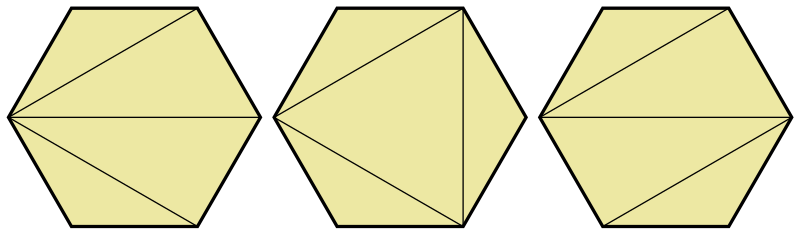
\includegraphics[width=0.5\textwidth]{images/polygons}
\caption{Πολύγωνα κατασκευασμένα από αρχέγονα}
\end{figure}

Η παρούσα εργασία αποτελεί προσπάθεια γενίκευσης και υλοποίησης της δοθείσας διαδικασίας \textlatin{triangle1} στην \textlatin{convex1}, η οποία χαράσσει αυθαίρετα κυρτά πολύγωνα, υπολογίζοντας αυξητικώς τις γραμμικές συναρτήσεις των ακμών τους για όλα τα εικονοστοιχεία του περιβάλλοντος κυτίου τους. Γενικώς τα τρίγωνα θεωρούνται αρχέγονα, διότι κάθε πολύγωνο δύναται να κατασκευαστεί από αυτά (Δρακόπουλος, 2021). Από πλευράς γεωμετρίας, ένα πολύγωνο (\textlatin{polygon}) είναι ένα επίπεδο σχήμα που ορίζεται από ένα σύνολο τριών ή περισσότερων θέσεων συντεταγμένων που ονομάζονται κορυφές (\textlatin{vertices}), και συνδέονται στη σειρά από ευθύγραμμα τμήματα που ονομάζονται ακμές (\textlatin{edges}) ή πλευρές (\textlatin{sides}) του πολυγώνου, οι οποίες δεν πρέπει να έχουν άλλα κοινά σημεία εκτός από τις κορυφές τους. Στην προκειμένη εργασία θα εξετάσουμε τα κυρτά πολύγωνα, τα οποία ορίζονται ως τα πολύγωνα των οποίων όλες οι εσωτερικές γωνίες είναι μικρότερες από ή ίσες με $180\degree$ (\textlatin{Hearn \& Baker, 2010}, σ. 117). \par

Η απεικόνιση των αρχεγόνων και κατ’ επέκταση των πολυγώνων γίνεται σε 2Δ συσκευές οθονών. Αυτές είναι διδιάστατες επιφάνειες πάνω στις οποίες προβάλλεται η οπτική πληροφορία ως ένα διακριτό πλέγμα εικονοστοιχείων. Η διαδικασία μετατροπής ενός 2Δ αρχεγόνου σε διακριτή αναπαράσταση εικονοστοιχείων, δηλαδή η εύρεση των εικονοστοιχείων  που απαρτίζουν ένα στοιχειώδες σχήμα, ονομάζεται ψηφιδόξυση ή χάραξη (\textlatin{rasterization}) (Δρακόπουλος, 2021?  Μουστάκας κ.ά., 2015? Σπύρου, 2019). \par

\chapter{Θεωρητικό υπόβαθρο}

Ένα απλό πολύγωνο είναι η περιοχή του επιπέδου που περικλείεται από ένα πεπερασμένο σύνολο ευθυγράμμων τμημάτων τα οποία σχηματίζουν μία κλειστή τεθλασμένη γραμμή. Τα $n$ ευθύγραμμα τμήματα αυτής της τμηματικώς γραμμικής καμπύλης αποτελούν τις ακμές του πολυγώνου και, σε συνδυασμό με τις $n$ κορυφές του, ορίζουν ένα πολυγωνικό πλέγμα ή μία πολυγωνική επιφάνεια. Στην πρώτη περίπτωση, σημεία του σχήματος θεωρούνται όσα σημεία ανήκουν στις ακμές, ενώ στη δεύτερη περίπτωση χρειάζεται ένας έλεγχος εσωτερικότητας των σημείων για να διαπιστωθεί αν αυτά ανήκουν στην επιφάνεια που ορίζεται από τις ακμές (Δρακόπουλος, 2021? Μουστάκας κ.ά., 2015? Παληός, 2021).

\section{Έλεγχος εσωτερικού σημείου}
Σύμφωνα με το θεώρημα καμπύλης \textlatin{Jordan (Jordan Curve Theorem)}, μία συνεχής, απλή, κλειστή και επίπεδη καμπύλη χωρίζει το επίπεδο σε δύο περιοχές, την εσωτερική (\textlatin{interior}) και την εξωτερική (\textlatin{exterior}) (Δρακόπουλος, 2021? Παληός, 2021). Οι αλγόριθμοι χάραξης πολυγώνων βασίζονται στον έλεγχο εσωτερικότητας κάθε σημείου του πολυγώνου. Οι κύριες μέθοδοι ελέγχου εσωτερικού σημείου είναι ο έλεγχος πλήθους συστροφών (\textlatin{winding number test}) και ο έλεγχος ισοτιμίας (\textlatin{parity test}). Συγκεκριμένα, ο δεύτερος έλεγχος πραγματοποιείται με τον σχεδιασμό ημιευθείας από το εικονοστοιχείο $p$ και την αρίθμηση του πλήθους των τομών της ημιευθείας με την περίμετρο του πολυγώνου $P$. Εφόσον ο αριθμός αυτός είναι περιττός, το $p$ είναι εσωτερικό του $P$; διαφορετικά, το $p$ είναι εξωτερικό του $P$ (Δρακόπουλος, 2021? Μουστάκας κ.ά., 2015).

\section{Ψηφιδόξυση πολυγώνου}
Ο βασικός αλγόριθμος ψηφιδόξυσης πολυγώνου βασίζεται στον έλεγχο ισοτιμίας. Ο αλγόριθμος υπολογίζει τις τομές $I(x, y)$ κάθε ακμής με όλες τις γραμμές διερεύνησης και τις αποθηκεύει σε μία κατάσταση, όπου πραγματοποείται η ταξινόμησή τους με κύριο κλειδί τη συντεταγμένη $y$ και δευτερεύον κλειδί τη συντεταγμένη $x$. Τέλος, εξάγει ζεύγη διαδοχικών σημείων τομής, τα οποία ονομάζονται εκτάματα και αντιπροσωπεύουν τις σειρές εικονοστοιχείων εσωτερικές του πολυγώνου (Δρακόπουλος, 2021? Σπύρου, 2019). \par

Ο παραπάνω αλγόριθμος δεν αποτελεί τη βέλτιστη μέθοδο ψηφιδόξυσης πολυγώνου, δεδομένου ότι η εύρεση του σημείου τομής είναι μία υπολογιστικά ακριβή πράξη. Μία αποδοτικότερη μέθοδος είναι ο αλγόριθμος χάραξης πολυγώνων κατά γραμμές διερεύνησης, ο οποίος εκμεταλλεύεται τη συνάφεια των γραμμών διερεύνησης και τη συνάφεια των ακμών που τέμνουν διαδοχικές γραμμές σάρωσης, και αποθηκεύει τις τομές της εκάστοτε γραμμής διερεύνησης σε μία δομή με τις ακμές του πολυγώνου. Ο αλγόριθμος χάραξης πολυγώνων κατά γραμμές διερεύνησης, η μέθοδος χάραξης με Πίνακα Ακμών και ο αλγόριθμος κρίσιμων σημείων, περιγράφονται αναλυτικά από τους Δρακόπουλο (2021, σ. 141-150), Μουστάκα και συνεργάτες (2015, σ. 40-42), και Σπύρου (2019, σ. 50-58).

\subsection{Αλγόριθμος χάραξης τριγώνου}
Όπως αναφέρθηκε στην \textbf{Εισαγωγή}, το τρίγωνο είναι το απλούστερο, επίπεδο, κυρτό πολύγωνο. Ένας τρόπος καθορισμού των εικονοστοιχείων τα οποία καλύπτουν ένα τρίγωνο είναι η εκτέλεση ελέγχου εσωτερικού σημείου σε όλα τα εικονοστοιχεία ευρισκόμενα εντός του περιβάλλοντος κυτίου του τριγώνου, δηλαδή του συνόλου έκτασης συντεταγμένων του τριγώνου, το οποίο περιέχει τις ελάχιστες και μέγιστες τιμές $x$, $y$ και $z$\footnote{Η πληροφορία υπεύθυνη για το χρώμα του εικονοστοιχείου αποθηκεύεται στη συντεταγμένη $z$.} του αντικειμένου (Δρακόπουλος, 2021? Σπύρου, 2019).

\subsection{Αλγόριθμος χάραξης κυρτού πολυγώνου}
Η χάραξη κυρτών πολυγώνων απαιτεί την υλοποίηση ενός παρόμοιου αλγορίθμου, εφόσον έχει πραγματοποιηθεί έλεγχος κυρτότητας των εν λόγω πολυγώνων. Μία χρήσιμη γεωμετρική δομή η οποία δύναται να διευκολύνει τον έλεγχο κυρτότητας πολυγώνων είναι το κυρτό περίβλημα (\textlatin{convex hull}). Το κυρτό περίβλημα ή κέλυφος ενός συνόλου σημείων $S$ στο επίπεδο ορίζεται ως το μικρότερο κυρτό πολύγωνο $Ρ$ που περικλείει το $S$, δηλαδή η τεθλασμένη γραμμή η οποία περικλείει πλήρως το σύνολο $S$, ώστε να εξαλείφονται οι κοιλότητες της γραμμής (Παληός, 2021, σ. 2? \textlatin{Sharma}, 2018). \par

\begin{figure}[h]
\centering
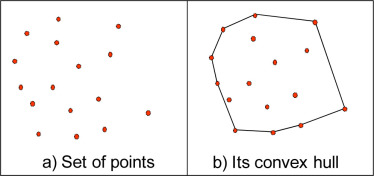
\includegraphics[width=0.5\textwidth]{images/convexhull}
\caption{Κυρτό περίβλημα ενός συνόλου σημείων}
\end{figure}

Οι πιο γνωστοί αλγόριθμοι εύρεσης του κυρτού περιβλήματος ενός πεπερασμένου συνόλου σημείων στο επίπεδο είναι ο αλγόριθμος σάρωσης του \textlatin{Graham (Graham’s scan}), ο αλγόριθμος περιτυλίγματος (\textlatin{Gift wrapping algorithm}) και ο αλγόριθμος του \textlatin{Chan},  όπως αυτοί περιγράφονται αναλυτικά από τους \textlatin{Graham (1972), Jarvis (1973)} και \textlatin{Chan (1996)} αντίστοιχα. Ο πρώτος αλγόριθμος υπολογίζει το κυρτό περίβλημα σε χρόνο $O(n \log n)$, ενώ ο δεύτερος έχει χρονική πολυπλοκότητα $O(nh)$, όπου $n$ το πλήθος των σημείων του επιπέδου και $h$ το πλήθος των απαιτούμενων επαναλήψεων για την εύρεση του κυρτού περιβλήματος. Ο τρίτος αλγόριθμος συνδυάζει τους δύο προηγούμενους ώστε να εξασφαλίσει μία χρονική πολυπλοκότητα $O(n \log h)$ (Κωστόπουλος, 2013).

\subsubsection{Αλγόριθμος περιτυλίγματος}
Δεδομένης της χρονικής πολυπλοκότητας του καθενός εκ των τριών προαναφερθέντων αλγορίθμων, ο αλγόριθμος περιτυλίγματος είναι ο βέλτιστος αλγόριθμος για την εύρεση του κυρτού περιβλήματος ενός περιορισμένου πλήθους σημείων $n$, ενώ αποτελεί χείριστη επιλογή όταν πρόκειται για ένα σημαντικό σύνολο σημείων $S$. \par

Η διαδικασία υπολογισμού ενός κυρτού περιβλήματος είναι ευκόλως ερμηνεύσιμη. Θέτοντας ως πρώτο σημείο $p_1$ του συνόλου $S$ το αριστερότερο σημείο, δηλαδή το σημείο ελάχιστης τιμής $x$, εντοπίζουμε το επόμενο σημείο $p_2$ το οποίο έχει ελάχιστη πολική γωνία $\geq 0$ του $p_1$. Ομοίως συγκρίνουμε σε χρόνο $O(n)$ τις πολικές γωνίες όλων των σημείων $n$ σε σχέση με το σημείο $p_i$ θεωρούμενο το κέντρο των πολικών συντεταγμένων, και επαναλαμβάνουμε τη διαδικασία $h$ φορές ωσότου $p_h=p_1$. Εν ολίγοις, ο εσωτερικός βρόχος ελέγχει κάθε σημείο του συνόλου $S$ και ο εξωτερικός βρόχος επαναλαμβάνεται για κάθε σημείο του περιβλήματος. Ως εκ τούτου, ο συνολικός χρόνος εκτέλεσης είναι $O(nh)$ και εξαρτάται από το μέγεθος της εξόδου, δηλαδή πρόκειται για έναν αλγόριθμο ευαίσθητο εξόδου\footnote{Αλγόριθμος ευαίσθητος εξόδου χαρακτηρίζεται ο αλγόριθμος του οποίου η χρονική πολυπλοκότητα εξαρτάται από το μέγεθος εξόδου του περιβλήματος.} (Κωστόπουλος, 2013? \textlatin{Jarvis, 1973}). \par

\pagebreak
\chapter{Υλοποίηση}

Έχοντας κατανοήσει τη θεωρία της γραφικής υπολογιστών και της υπολογιστικής γεωμετρίας αναφορικά με την χάραξη πολυγώνων, είμαστε σε θέση να ερμηνεύσουμε τον δοθέντα αλγόριθμο χάραξης τριγώνου και να τον γενικεύσουμε σε έναν αλγόριθμο χάραξης κυρτών πολυγώνων.

\section{Επεξήγηση διαδικασίας \textlatin{triangle1}}
H διαδικασία \textlatin{triangle1} περιγράφει έναν απλό αλγόριθμο ψηφιδόξυσης τριγώνου. Η συνάρτηση δέχεται ως ορίσματα τις τρεις κορυφές του τριγώνου και την τιμή χρωματισμού των εικονοστοιχείων ευρισκόμενων εντός του πολυγώνου. Αφού αρχικοποιήσουμε τις μεταβλητές των ακμών και των γραμμικών συναρτήσεων, καλούμε την κατάλληλη συνάρτηση για να σχεδιάσουμε τις ακμές του τριγώνου. Ακολουθεί ο υπολογισμός του περιβάλλοντος κυτίου του τριγώνου, η εκτίμηση των γραμμικών συναρτήσεων στο κατώτερο σημείο του, και η αποθήκευσή τους στις αντίστοιχες προσωρινές μεταβλητές, με σκοπό τον έλεγχο των προσήμων των συναρτήσεων και κατ’ επέκταση τον προσδιορισμό της θέσης κάθε εικονοστοιχείου. Για κάθε εικονοστοιχείο $p$ του περιβάλλοντος κυτίου, εάν οι τιμές και των τριών συναρτήσεων έχουν το ίδιο πρόσημο, τότε το $p$ ευρίσκεται εντός του τριγώνου, αλλιώς ευρίσκεται εκτός αυτού (Δρακόπουλος, 2021, σ. 152? Σπύρου, 2019, σ. 60). Για ομόσημες γραμμικές συναρτήσεις, καλούμε τη συνάρτηση χρωματισμού εικονοστοιχείου και, μέσω του διπλού βρόχου επανάληψης, επιτυγχάνεται τελικώς η ψηφιδόξυση του τριγώνου.

\section{Γενίκευση διαδικασίας \textlatin{triangle1} στην \textlatin{convex1}}
Εφόσον κάθε πολύγωνο δύναται να κατασκευαστεί από τρίγωνα, η διαδικασία χάραξης τριγώνων \textlatin{triangle1} δύναται να γενικευθεί παρομοίως στη διαδικασία χάραξης κυρτών πολυγώνων \textlatin{convex1}. Αρχικά, η συνάρτηση \textlatin{convex1} δέχεται ως ορίσματα την τιμή χρωματισμού των εικονοστοιχείων ευρισκόμενων εντός του πολυγώνου, και ένα πλήθος σημείων $S$ ορισμένο από τον χρήστη. Κατόπιν, αρχικοποιούνται οι απαραίτητες μεταβλητές για τον έλεγχο κυρτότητας, τον σχεδιασμό ακμών και τον υπολογισμό των γραμμικών συναρτήσεων του πολυγώνου. \par

Η επιλογή του αλγορίθμου περιτυλίγματος για τον έλεγχο κυρτότητας του πολυγώνου βασίζεται στην προμελετηθείσα θεωρία. Ο αλγόριθμος υλοποιείται καλώντας τη συνάρτηση \textlatin{jarvis} με όρισμα το μέγεθος του πίνακα σημείων στο επίπεδο, δηλαδή το σύνολο των δυνητικών κορυφών του πολυγώνου. Αρχικά, αποθηκεύουμε την τιμή του αριστερότερου σημείου του συνόλου στη μεταβλητή $leftPoint$, και υλοποιούμε τον διπλό βρόχο επανάληψης του αλγορίθμου περιτυλίγματος. Συγκεκριμένα, ορίζουμε το $p[i]$ ως το αριστερότερο σημείο του επιπέδου, και επιλέγουμε αυθαίρετα ως τελικό σημείο $endPoint$ το πρώτο σημείο του συνόλου $S$. Στον εσωτερικό βρόχο ελέγχουμε εάν το τελικό σημείο και το αριστερότερο σημείο ταυτίζονται, ή εάν το τρέχον σημείο που εξετάζεται είναι αριστερότερα του $leftPoint$. Αν ισχύει οιαδήποτε εκ των δύο συνθηκών, θέτουμε το τελικό σημείο ίσο με το τρέχον σημείο και καλούμε την κατάλληλη συνάρτηση για τη σχεδίαση των ακμών, ενώ στον εξωτερικό βρόχο αποθηκεύουμε την τιμή του τελικού σημείου στη θέση του αριστερότερου σημείου. Οι επαναλήψεις τερματίζουν όταν το τελικό σημείο ταυτιστεί με το πρώτο σημείο του πολυγώνου, δηλαδή όταν η πολυγωνική αλυσίδα των κορυφών κλείσει και σχηματίσει το κυρτό περίβλημα (Κωστόπουλος, 2013? \textlatin{Jarvis, 1973; Sharma, 2018}). \par

\begin{figure}[h]
\centering
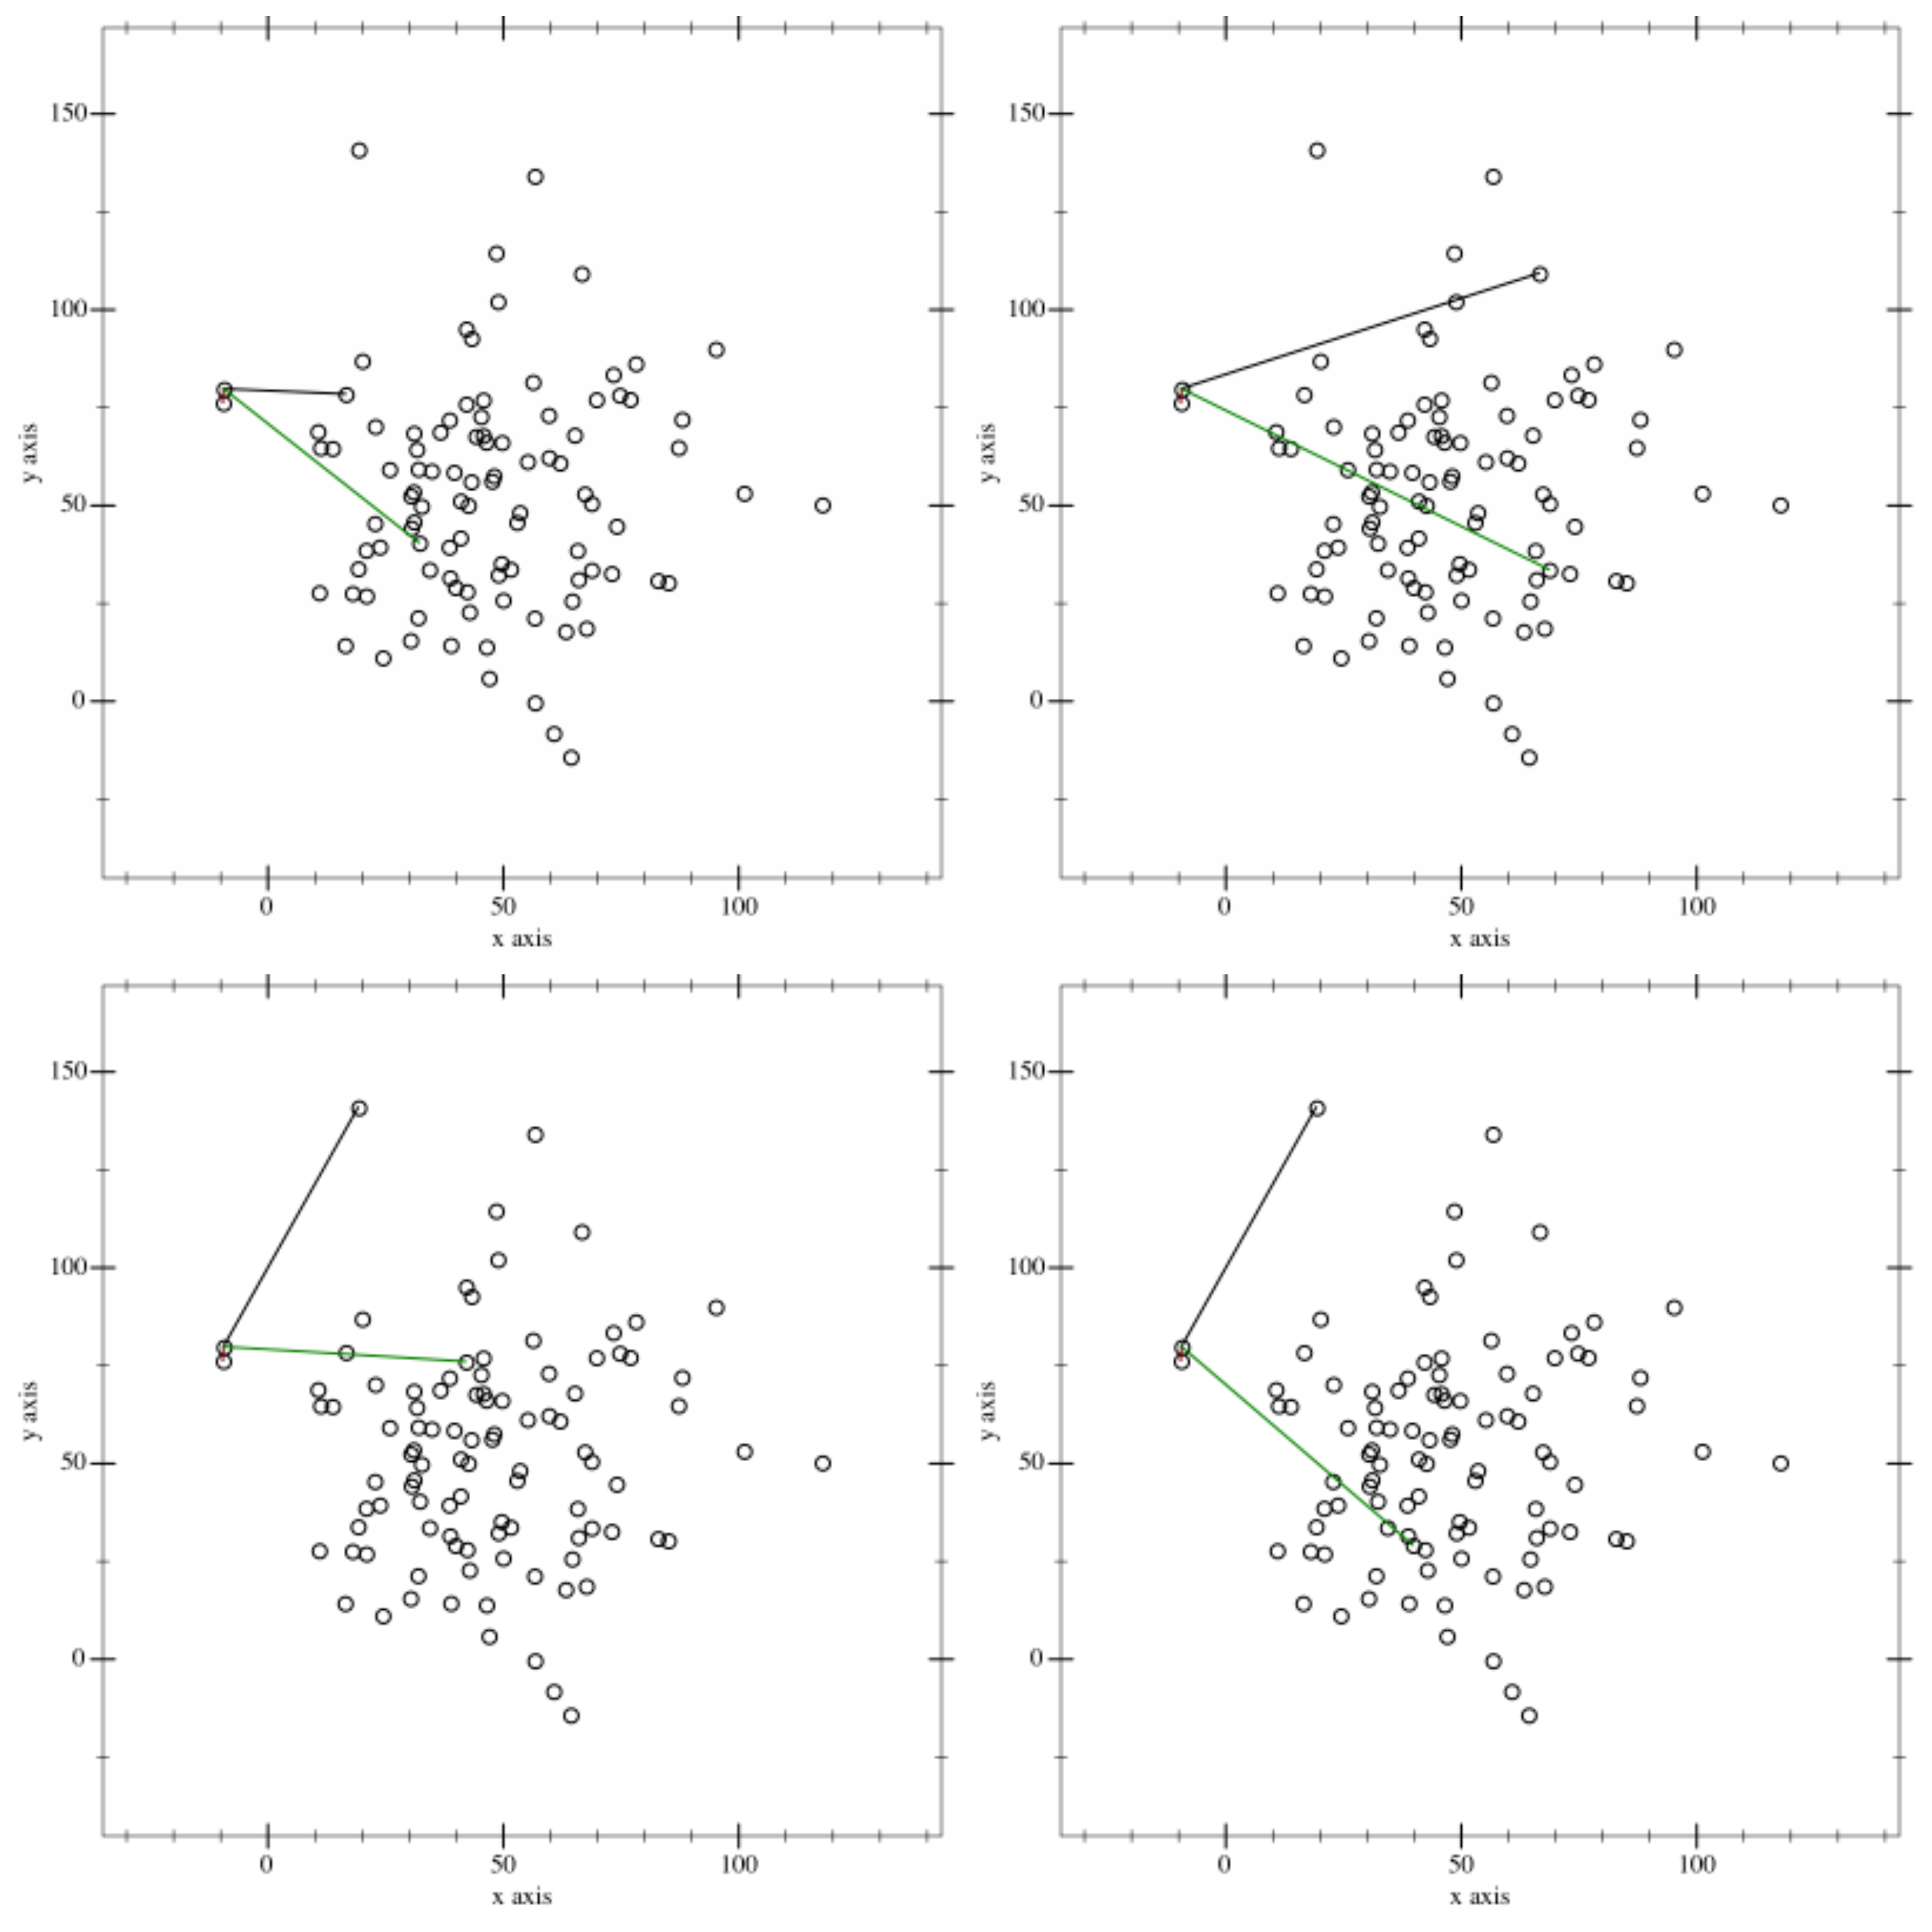
\includegraphics[width=0.45\textwidth]{images/jarvis}
\caption{Στιγμιότυπα εκτέλεσης του αλγορίθμου περιτυλίγματος (\textlatin{Sharma}, 2018)}
\end{figure}

Η υπόλοιπη διαδικασία\footnote{Υπολογισμός του περιβάλλοντος κυτίου του πολυγώνου, εκτίμηση των γραμμικών συναρτήσεων στο σημείο $bb\_xmin, bb\_ymin$, έλεγχος προσήμων των γραμμικών συναρτήσεων} \textlatin{convex1} ακολουθεί τα βήματα της \textlatin{triangle1}, χρησιμοποιώντας πίνακες αποθήκευσης των κορυφών, των ακμών και των γραμμικών συναρτήσεων, και καλώντας βρόχους επανάληψης για την υλοποίηση των πράξεων, δεδομένου ότι δεν αφορά γνωστό πλήθος κορυφών, αλλά αυθαίρετα παραγόμενο σύνολο σημείων στο επίπεδο. \par

\subsection{Υλοποίηση σε \textlatin{OpenGL}}

Tμήμα της υλοποίησης εκφράστηκε στη γλώσσα προγραμματισμού \textlatin{C++} με τη βοήθεια της \textlatin{OpenGL}. Η \textlatin{OpenGL} αποτελεί πρότυπο καθορισμού λειτουργιών που πρέπει να υποστηρίζει μια βιβλιοθήκη γραφικών για να είναι συμβατή με αυτήν. Είναι ανεξάρτητη λειτουργικού συστήματος και ορίζει µια προγραµµατιστική διεπιφάνεια σχεδίασης γραφικών (Δρακόπουλος, 2022). \par

Ο εκτελέσιμος κώδικας περιέχει συναρτήσεις \textbf{\textlatin{void}} για τη χάραξη κυρτού πολυγώνου και τη δημιουργία σχήματος με την χρήση του ποντικιού. Αναλυτικότερα, στο πεδίο της \textbf{\textlatin{void mouse}} ορίζεται η κλήση του ποντικιού για το τρέχον παράθυρο και με κάθε πάτημα-απελευθέρωσή του, αποστέλλονται σήματα που υποδεικνύουν τις συντεταγμένες $x$ και $y$ των κορυφών του πολυγώνου. Κατά την \textbf{\textlatin{void display}} ορίζεται το χρώμα σχεδίασης και η δημιουργία του πολυγώνου βάσει των εντολών που αναγράφονται στον παρακάτω πίνακα, καθώς και στο αρχείο του κώδικα. Τελικώς, οι παραπάνω συναρτήσεις καλούνται στην \textbf{\textlatin{main}} συνάρτηση του προγράμματος για την ψηφιδόξυση πολυγώνων με κορυφές ορισμένες από την αλληλεπίδραση του χρήστη με το παράθυρο εφαρμογής. \par

\vspace{2em}

\begin{center}
    \begin{longtable}{p{6.5cm}|p{7cm}} 
        \textbf{Εντολές} & \textbf{Εξήγηση} \\ \hline \hline
        \textlatin{\lstinline[language=C]!void mouse()!} & Συνάρτηση διαχείρισης σημάτων από το ποντίκι \\ \hline
        \textlatin{\lstinline[language=C]!GLUT_LEFT_BUTTON / GLUT_UP!} & Λήψη σήματος κατά την απελευθέρωση του αριστερού κουμπιού του ποντικιού \\ \hline
        \textlatin{\lstinline[language=C]!void display()!} & Συνάρτηση που διαχειρίζεται τι σχεδιάζεται στην οθόνη και με ποια σειρά \\ \hline
        \textlatin{\lstinline[language=C]!glColor3f(1, 0, 0)!} & Επιλογή χρώµατος σχεδίασης (κόκκινο) \\ \hline
        \textlatin{\lstinline[language=C]!glMatrixMode(GL_PROJECTION)!}  & Επιλογή μητρώου προβολής \\ \hline
        \textlatin{\lstinline[language=C]!glLoadIdentity!} & Αντικατάσταση τρέχοντος μητρώου από το μητρώο προβολής \\ \hline
        \textlatin{\lstinline[language=C]!gluOrtho2D(0, 640, 0, 480)!} & Δήλωση παράλληλης προβολής \\
        \hline
        \textlatin{\lstinline[language=C]!glBegin(GL_POLYGON) / glEnd!} & Μεταξύ αυτών των εντολών δηλώνονται συντεταγµένες κορυφών κυρτού πολυγώνου \\ \hline
        \textlatin{\lstinline[language=C]!glVertex2f(x, y)!} & Δήλωση συντεταγµένων μεμονομένων κορυφών (δύο παράμετροι τύπου \textlatin{float}) \\ \hline
        \textlatin{\lstinline[language=C]!glFlush!} & Προώθηση εκτέλεσης εκκρεμούντων εντολών \\ \hline
        \textlatin{\lstinline[language=C]!glutInitWindowSize(640, 480)!} & Ορισμός διαστάσεων παραθύρου εφαρµογής σε \textlatin{pixels} \\ \hline
        \textlatin{\lstinline[language=C]!glutInitWindowPosition(100, 100)!} & Δήλωση θέσης παραθύρου εφαρμογής στην οθόνη \\ \hline
        \textlatin{\lstinline[language=C]!glutInitDisplayMode!} & Καθορίζει ρυθµίσεις απεικόνισης (µοντέλο ενταµίευσης, χρωµατικό µοντέλο κ.λ.π.) \\ \hline
        \textlatin{\lstinline[language=C]!GLUT_SINGLE | GLUT_RGB!} & Δήλωση μοντέλου απλής ενταμίευσης (\textlatin{single buffer}) και χρωματικού μοντέλου \textlatin{RGB} \\ \hline
        \textlatin{\lstinline[language=C]!glutCreateWindow("Convex1")!} & Εµφάνιση παραθύρου εφαρµογής \\ \hline
        \textlatin{\lstinline[language=C]!glClearColor(1,1,1,0)!} & Δήλωση χρώµατος καθαρισµού της οθόνης (λευκό) \\ \hline
        \textlatin{\lstinline[language=C]!glClear!} & Καθαρισµός ενός από τους ενταµιευτές του συστήµατος γραφικών \\ \hline
        \textlatin{\lstinline[language=C]!glutDisplayFunc(display)!} & Κλήση συνάρτησης σχεδιασμού της σκηνής \\ \hline
        \textlatin{\lstinline[language=C]!glutMouseFunc(mouse)!} & Κλήση συνάρτησης αλληλεπίδρασης με το ποντίκι \\ \hline
        \textlatin{\lstinline[language=C]!glutMainLoop()!} & Ενεργοποίηση κύκλου ακρόασης γεγονότων \\ \hline
    \caption{Πίναξ εντολών \textlatin{OpenGL}}
    \end{longtable}
\end{center}

% Συμπεράσματα

\addcontentsline{toc}{chapter}{Συμπεράσματα}
\chapter*{Συμπεράσματα}

Όπως έχει ήδη αναφερθεί, σκοπός της παρούσας εργασίας ήταν η γενίκευση και υλοποίηση της διαδικασίας \textlatin{triangle1} στην \textlatin{convex1}, η οποία χαράσσει αυθαίρετα κυρτά πολύγωνα, υπολογίζοντας αυξητικώς τις γραμμικές συναρτήσεις των ακμών τους για όλα τα εικονοστοιχεία του περιβάλλοντος κυτίου τους. Διαπιστώσαμε πως η γενίκευση της διαδικασίας \textlatin{triangle1} είναι εφικτή και δύναται να υλοποιηθεί με μία πληθώρα διαφορετικών μεθόδων, αναλόγως τις απαιτήσεις του χρήστη. Επιπρόσθετα, παρ’ όλο που η διαδικασία υλοποιήθηκε βάσει του αλγορίθμου περιτυλίγματος, αναγνωρίζουμε ότι η χρονική πολυπλοκότητα της χειρότερης περίπτωσης του εν λόγω αλγορίθμου τον καθιστά μη αποδοτικό για μεγάλο όγκο σημείων ενός κυρτού πολυγώνου.  \par

Δοθέντος αρκετού χρόνου για εμβάθυνση στο θέμα της εργασίας και εξοικείωση με την προγραμματιστική πλατφόρμα \textlatin{OpenGL}, στοχεύουμε στην εκτενέστερη εξέταση και την βελτιστοποίηση των υλοποιημένων αλγορίθμων ψηφιδόξυσης κυρτών πολυγώνων με τη χρήση του προαναφερθέντος λογισμικού. Στους μελλοντικούς μας στόχους συμπεριλαμβάνεται και η μελέτη των υπολοίπων αλγορίθμων χάραξης πολυγώνων που αναφέρθηκαν στο πλαίσιο της παρούσας εργασίας.

% Επίλογος

\addcontentsline{toc}{chapter}{Επίλογος}
\chapter*{Επίλογος}

Εν κατακλείδι, η γενίκευση της διαδικασίας \textlatin{triangle1} στην \textlatin{convex1} για την χάραξη αυθαίρετων κυρτών πολυγώνων, υλοποιήθηκε με επιτυχία και έθεσε νέους στόχους και ερωτήματα αναφορικά με τις προοπτικές του κάθε αλγόριθμου ψηφιδόξυσης, τόσο στις δύο διαστάσεις όσο και στις τρεις.
\newpage
% Αναφορές

\addcontentsline{toc}{chapter}{Αναφορές}

\begin{thebibliography}{16}

% Ελληνόγλωσση βιβλιογραφία

\bibitem{1} Δρακόπουλος, Β. (2021). \emph{Εισαγωγή και Αλγόριθμοι ψηφιδόξυσης} [Πανεπιστημιακές Σημειώσεις]. Πανεπιστήμιο Θεσσαλίας, Τμήμα Πληροφορικής με Εφαρμογές στη Βιοϊατρική, Π.Π.Σ.: "Γραφική Υπολογιστών", Εαρινό Εξάμηνο 2020-2021, Λαμία

\bibitem{2} Μουστάκας, Κ., Παλιόκας, Ι., Τζοβάρας, Δ., \& Τσακίρης, Α. (2015). \textit{Γραφικά και Εικονική Πραγματικότητα} [ηλεκτρ. βιβλ.]. Αθήνα: Σύνδεσμος Ελληνικών Ακαδημαϊκών Βιβλιοθηκών. \textlatin{\url{http://hdl.handle.net/11419/4491}}

\bibitem{3} Σπύρου, Ε. (2019). \emph{Αλγόριθμοι Σχεδίασης} [Πανεπιστημιακές Σημειώσεις]. Πανεπιστήμιο Θεσσαλίας, Τμήμα Πληροφορικής και Τηλεπικοινωνιών, Π.Π.Σ.: "Γραφικά", Εαρινό Εξάμηνο 2018-2019, Λαμία

\bibitem{4} Παληός, Λ. (2021). \emph{1. Διαίρεση Πολυγώνων σε Τρίγωνα, 2. Το πρόβλημα του Κυρτού Πολυγώνου στις Δύο Διαστάσεις} [Πανεπιστημιακές Σημειώσεις]. Πανεπιστήμιο Ιωαννίνων, Τμήμα Μηχανικών Η/Υ και Πληροφορικής, Π.Π.Σ.: "Υπολογιστική Γεωμετρία", Εαρινό Εξάμηνο 2020-2021, Ιωάννινα

\bibitem{5} Κωστόπουλος, Π. (2013). \emph{Μέθοδοι κατασκευής κυρτών περιβλημάτων και εφαρμογές}. [Μεταπτυχιακή Εργασία]. Αμητός: Αποθετήριο Πανεπιστημίου Πελοποννήσου. \textlatin{\url{https://amitos.library.uop.gr/xmlui/handle/123456789/980}}.

\bibitem{6} \textlatin{Hearn, D., \& Baker, M. P.} (2010). \emph{Γραφικά Υπολογιστών με \textlatin{OpenGL}} (Π. Μποζάνης, Επιμ.) (Γ. Σίσιας, Μετάφ.) (3η έκδ.). Θεσσαλονίκη: ΤΖΙΟΛΑ. (Το πρωτότυπο έργο δημοσιεύτηκε το 1986).

\bibitem{7} Δρακόπουλος, Β. (2022). \emph{Εισαγωγή στην \textlatin{OpenGL}} [Εργαστηριακές Σημειώσεις]. Πανεπιστήμιο Θεσσαλίας, Τμήμα Πληροφορικής με Εφαρμογές στη Βιοϊατρική, Π.Π.Σ.: "Γραφική Υπολογιστών", Εαρινό Εξάμηνο 2021-2022, Λαμία

\bibitem{8} Εργαστήριο Τεχνολογίας Πολυμέσων (\textlatin{medialab}) (2017). \emph{Κεφάλαιο 1: Βασικές αρχές σχεδίασης} [Πανεπιστημιακές Σημειώσεις]. Εθνικό Μετσόβιο Πολυτεχνείο, Τμήμα Ηλεκτρολόγων Μηχανικών και Μηχανικών Υπολογιστών, Αθήνα. Ανακτήθηκε από: \textlatin{\url{ http://www.medialab.ntua.gr/education/ComputerGraphics/OpenGL_Lectures/02-Chapter1.pdf}}

\vspace{2.5em}

% Ξενόγλωσση βιβλιογραφία

\bibitem{9} \textlatin{Kjeldsen, T. H. (2010). History of convexity and mathematical programming: connections and relationships in two episodes of research in pure and applied mathematics of the 20th century. In R. Bhatia (Ed.), \emph{Proceedings of the International Congress of Mathematicians 2010 - Invited lectures}, 4, 3233-3257. Hindustan Book Agency.}

\bibitem{10} \textlatin{Graham, R.L. (1972). An efficient algorithm for determining the convex hull of a finite planar set. \emph{Information Processing Letters}, 1(4), 132–133. doi: 10.1016/0020-0190(72)90045-2.}

\bibitem{11} \textlatin{Jarvis, R. A. (1973). On the identification of the convex hull of a finite set of points in the plane. \emph{Information Processing Letters}, 2(1), 18-21. doi: 10.1016/0020-0190(73)90020-3.}

\bibitem{12} \textlatin{Chan, T.M. (1996). Optimal output-sensitive convex hull algorithms in two and three dimensions. \emph{Discrete \& Computational Geometry}, 16, 361–368. doi: 10.1007/BF02712873.}

\bibitem{13} \textlatin{Sharma, P. (2018, July 2). Gift Wrap Algorithm (Jarvis March Algorithm) to find Convex Hull. \emph{OpenGenus IQ: Learn Computer Science}}. Ανακτήθηκε από: \textlatin{\url{https://iq.opengenus.org/gift-wrap-jarvis-march-algorithm-convex-hull/}}

\bibitem{14} \textlatin{Neider, J., \& Davis, T. (1997). \emph{Opengl Programming Guide: The Official Guide to Learning Opengl, Version 1.1, Second Edition}. Addison-Wesley Publishing Company.} Ανακτήθηκε από: \textlatin{\url{http://www.cse.chalmers.se/edu/course/TDA362/redbook.pdf}}

\bibitem{15} \textlatin{Wang, Y. F. (2017). \emph{OpenGL Input}} [Πανεπιστημιακές Σημειώσεις]. \textlatin{University of California, Computer Science Department}, Π.Π.Σ.: \textlatin{"Introduction to Computer Graphics"}, Χειμερινό Εξάμηνο 2017-2018, \textlatin{Santa Barbara}

\bibitem{16} \textlatin{Agu, E. O. (2016). \emph{Lecture 3: Introduction to OpenGL/GLUT (Part 2)}} [Πανεπιστημιακές Σημειώσεις]. \textlatin{Worcester Polytechnic Institute (WPI), Computer Science Department}, Π.Π.Σ.: \textlatin{"Computer Graphics"}, Εαρινό Εξάμηνο 2016, \textlatin{Worcester}

\end{thebibliography}


\end{document}
